% Standalone source of Fig. 1 (compiled separately; the ieeeaccess class
% redefines \year, which breaks TikZ when it is loaded in the main document).
\documentclass[border=2pt]{standalone}
\usepackage{mathptmx}
\usepackage{tikz}
\usetikzlibrary{arrows.meta,positioning,fit,backgrounds,calc}
\newcommand{\clir}{CLIR}
\begin{document}
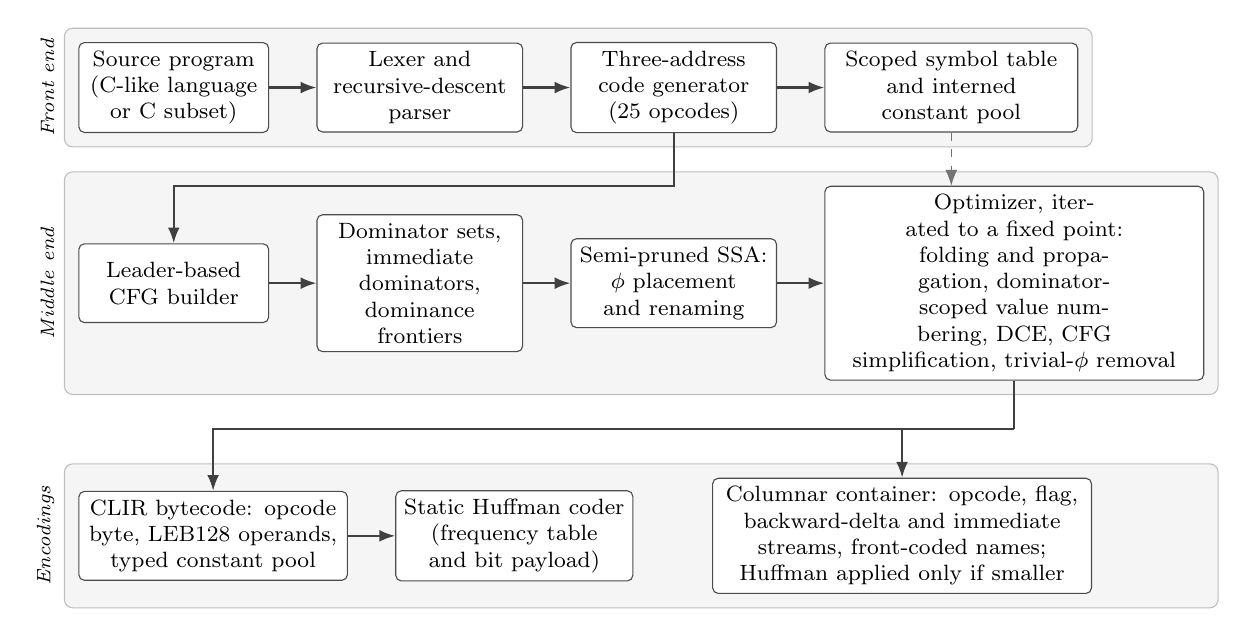
\begin{tikzpicture}[
  font=\footnotesize,
  box/.style={draw=black!70, rounded corners=2pt, align=center, minimum height=10mm,
              inner sep=3pt, fill=white},
  lane/.style={draw=black!25, rounded corners=3pt, fill=black!4, inner sep=5pt},
  arr/.style={-{Latex[length=2mm]}, black!75, thick},
  side/.style={-{Latex[length=2mm]}, black!55, dashed}]
  % ---------------- front end
  \node[box, text width=22mm] (src) {Source program\\(C-like language\\or C subset)};
  \node[box, text width=24mm, right=6mm of src] (parse) {Lexer and\\recursive-descent\\parser};
  \node[box, text width=24mm, right=6mm of parse] (tac) {Three-address\\code generator\\(25 opcodes)};
  \node[box, text width=30mm, right=6mm of tac] (tabs) {Scoped symbol table\\and interned\\constant pool};
  % ---------------- middle end
  \node[box, text width=22mm, below=14mm of src] (cfg) {Leader-based\\CFG builder};
  \node[box, text width=24mm, right=6mm of cfg] (dom) {Dominator sets,\\immediate dominators,\\dominance frontiers};
  \node[box, text width=24mm, right=6mm of dom] (ssa) {Semi-pruned SSA:\\$\phi$ placement\\and renaming};
  \node[box, text width=46mm, right=6mm of ssa] (opt) {Optimizer, iterated to a fixed point:\\folding and propagation, dominator-\\scoped value numbering, DCE, CFG\\simplification, trivial-$\phi$ removal};
  % ---------------- encodings
  \node[box, text width=32mm, anchor=north west] (clir) at ($(cfg.west |- opt.south)+(0,-14mm)$)
       {\clir{} bytecode: opcode\\byte, LEB128 operands,\\typed constant pool};
  \node[box, text width=28mm, right=6mm of clir] (huff) {Static Huffman coder\\(frequency table\\and bit payload)};
  \node[box, text width=46mm, right=10mm of huff] (soa) {Columnar container: opcode, flag,\\backward-delta and immediate\\streams, front-coded names;\\Huffman applied only if smaller};
  % ---------------- program flow
  \draw[arr] (src) -- (parse);
  \draw[arr] (parse) -- (tac);
  \draw[arr] (tac) -- (tabs);
  \coordinate (bus1) at ($(tac.south)!0.5!(ssa.north)$);
  \draw[arr] (tac.south) -- (tac.south |- bus1) -| (cfg.north);
  \draw[arr] (cfg) -- (dom);
  \draw[arr] (dom) -- (ssa);
  \draw[arr] (ssa) -- (opt);
  \coordinate (bus2) at ($(opt.south)!0.5!(soa.north)$);
  \draw[black!75, thick] (opt.south) -- (opt.south |- bus2);
  \draw[arr] (opt.south |- bus2) -| (clir.north);
  \draw[arr] (opt.south |- bus2) -| (soa.north);
  \draw[arr] (clir) -- (huff);
  % ---------------- side information
  \draw[side] (tabs.south) -- (tabs.south |- opt.north);
  % ---------------- lanes
  \begin{scope}[on background layer]
    \node[lane, fit=(src)(tabs), label={[font=\scriptsize\itshape, rotate=90, anchor=south]left:Front end}] {};
    \node[lane, fit=(cfg)(opt), label={[font=\scriptsize\itshape, rotate=90, anchor=south]left:Middle end}] {};
    \node[lane, fit=(clir)(soa)(opt.east |- soa.east), label={[font=\scriptsize\itshape, rotate=90, anchor=south]left:Encodings}] {};
  \end{scope}
\end{tikzpicture}
\end{document}
